\documentclass[12pt, letterpaper, oneside]{article}		% article class
\usepackage[parfill]{parskip}   						% Begin paragraphs with empty line rather than an indent
\usepackage{amsmath} 							% Align
\usepackage{graphicx}							% Figure
\usepackage[colorlinks=true, urlcolor=blue]{hyperref}	% Hyperlinks
\usepackage{listings}							% Code highlighting
\usepackage{color}								% Background of code
\setcounter{tocdepth}{4}							% Table of contents to level 5 (Paragraph)
\setcounter{secnumdepth}{2}						% Only number down to section level

% http://en.wikibooks.org/wiki/LaTeX/Packages/Listings
\lstset{ %
	   backgroundcolor=\color{white},
	   breakatwhitespace=true, 
	   commentstyle=\color{green}
	   keepspaces=false
	   language=IDL, 
	   showspaces=false			% True -> puts an underscore at all of the spaces.
	 }

% See the ``Article customise'' template for come common customisations

\title{MrWindow}
\author{Matthew Argall}
%\date{}

%%% BEGIN DOCUMENT
\begin{document}

\maketitle
\tableofcontents

% COPYRIGHT
\section{Copyright}
\label{sec: copyright}

This work is copyrighted under the New BSD license.

Copyright (c) 2013, Matthew Argall. All rights reserved.

Redistribution and use in source and binary forms, with or without modification, are permitted provided that the following conditions are met:

\begin{enumerate}
	\item Redistributions of source code must retain the above copyright notice, this list of conditions and the following disclaimer.
	\item Redistributions in binary form must reproduce the above copyright notice, this list of conditions and the following disclaimer in the documentation and/or other materials provided with the distribution.
	\item Neither the name of the <ORGANIZATION> nor the names of its contributors may be used to endorse or promote products derived from this software without specific prior written permission.
\end{enumerate}

THIS SOFTWARE IS PROVIDED BY THE COPYRIGHT HOLDERS AND CONTRIBUTORS "AS IS" AND ANY EXPRESS OR IMPLIED WARRANTIES, INCLUDING, BUT NOT LIMITED TO, THE IMPLIED WARRANTIES OF MERCHANTABILITY AND FITNESS FOR A PARTICULAR PURPOSE ARE DISCLAIMED. IN NO EVENT SHALL THE COPYRIGHT HOLDER OR CONTRIBUTORS BE LIABLE FOR ANY DIRECT, INDIRECT, INCIDENTAL, SPECIAL, EXEMPLARY, OR CONSEQUENTIAL DAMAGES (INCLUDING, BUT NOT LIMITED TO, PROCUREMENT OF SUBSTITUTE GOODS OR SERVICES; LOSS OF USE, DATA, OR PROFITS; OR BUSINESS INTERRUPTION) HOWEVER CAUSED AND ON ANY THEORY OF LIABILITY, WHETHER IN CONTRACT, STRICT LIABILITY, OR TORT (INCLUDING NEGLIGENCE OR OTHERWISE) ARISING IN ANY WAY OUT OF THE USE OF THIS SOFTWARE, EVEN IF ADVISED OF THE POSSIBILITY OF SUCH DAMAGE.

%GETTING STARTED
\section{Getting Started}
\label{sec: getting started}

The first step is to let IDL know where MrWindow is. There are several options.

\begin{enumerate}
	\item Restore `MrWindow.sav' 
	
\begin{lstlisting}
restore, `[path_to_MrWindow_Directory]/MrWindow.sav'
\end{lstlisting}

	\item Compile all of the files individually
        	\begin{enumerate}
		\item Change directories to the MrWindow directory
        		\item Start idl with the following command:
	
\begin{lstlisting}
idl compile_mrwindow
\end{lstlisting}
                		
	\end{enumerate}
	\item Add the MrWindow directory and its subdirectories to the IDL path
        	\begin{enumerate}
		\item Unix:
	
\begin{lstlisting}
!path + `:' + expand_path(`+/[path]/MrWindow/')
\end{lstlisting}
	
               
        		\item Windows:
	
\begin{lstlisting}
!path = !path + `;' + expand_path(`+[path]\MrWindow\')
\end{lstlisting}
	
                
	\end{enumerate}
	\item Edit the system variable \verb IDL_PATH  to include the MrWindow directory
	\item Create a \verb startup.pro  file containing the lines in step (2)
\end{enumerate}

%THOROUGH EXAMPLE
\section{Thorough Example}
\label{sec: Thorough Example}

The goal of this example is to show how easy it is to add plottable objects to a MrWindow window. These objects can be manipulatd in many useful ways.

%Creating an empty MrWindow
\subsection{Creating an empty MrWindow}

It is easy to create a new MrWindow. Just type:

\begin{lstlisting}
    myWindow = obj_new('MrWindow')
\end{lstlisting}

\begin{figure}[h!]
  \centering
  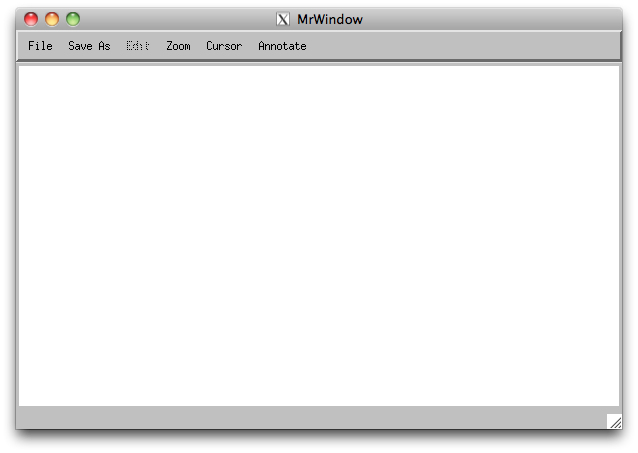
\includegraphics[width=0.4 \textwidth]{./figures/MrWindow_new.png}
  \caption[A new MrWindow.]
   {A new MrWindow.}
\end{figure}


%Plot a sine wave
\subsection{Plot a Sine Wave}

\begin{lstlisting}
    x = findgen(101)/100
    y = sin(2*!pi*x)
    myWindow -> Plot, x, y, TITLE='Sin(x)', YTITLE='Amplitude', XTITLE='Time (s)'
\end{lstlisting}

\begin{figure}[h!]
  \centering
  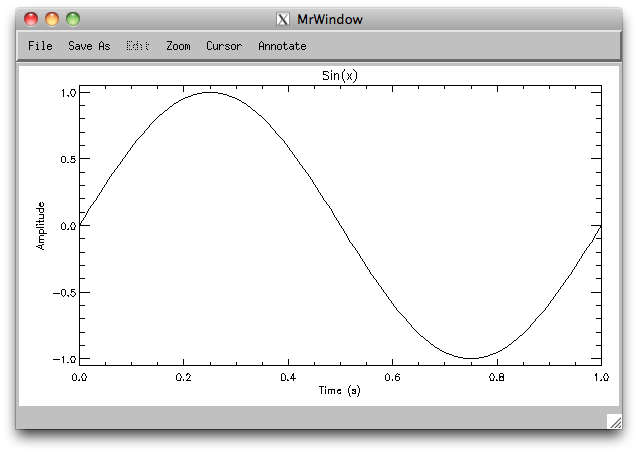
\includegraphics[width=0.5 \textwidth]{./figures/Sine-wave.png}
  \caption[Sin(x) in MrWindow.]
   {A sine wave has now been added to the MrWindow object.}
\end{figure}

%Add another plot
\subsection{Add Another Plot}

\begin{lstlisting}
x = findgen(101)/100
y = sin(2*!pi*x)
myWindow -> Plot, x, y, TITLE='Oops! Wrong Title', YTITLE='Amplitude', XTITLE='Time (s)'
\end{lstlisting}

\begin{figure}[h!]
  \centering
  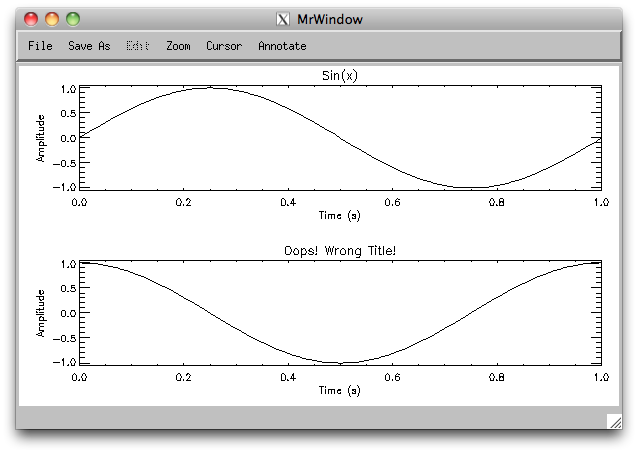
\includegraphics[width=0.5 \textwidth]{./figures/Sine-Cosine-Wrong-Title.png}
  \caption[Add a Cosine Wave.]
   {A cosine wave has been added and the sine wave has been moved so that both can fit.}
\end{figure}

%Change Plot Properties
\subsection{Changing Plot Properties}

\begin{lstlisting}
    ;First we need to know the index at which the plot is stored.
    myWindow -> whichObjects
\end{lstlisting}

\begin{figure}[h!]
  \centering
  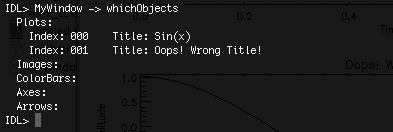
\includegraphics[width=0.75 \textwidth]{./figures/whichObjects.png}
  \caption[whichObjects.]
   {whichObjects shows all of the objects that are displayed, some identifying information, and the index at which they are stored.}
\end{figure}

\begin{lstlisting}
;It is at index 1 and it is a plot
myWindow -> SetProperty, 1, /PLOT, TITLE='Cos(x)', XRANGE=[0.25, 0.75], XSTYLE=1, /DRAW
\end{lstlisting}

\begin{figure}[h!]
  \centering
  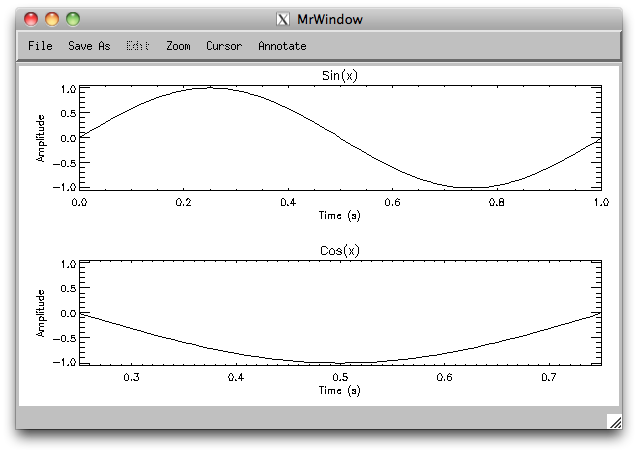
\includegraphics[width=0.75 \textwidth]{./figures/Sine-Cosine-Correct-Title.png}
  \caption[Title Change.]
   {Several properties of the Cosine plot have been changed. Now the title is correct!.}
\end{figure}

%Bind Axes
\subsection{Bind Axes}
; 5. Get the object references for each plot and bind their x-axes together so that zoom
;    events for one plot apply to all of the bound plots.
   
\begin{lstlisting}
;Get the object reference for each (they are at indices 0 and 1)
myWindow -> GetProperty, 0, /PLOT, OREF=oSin
myWindow -> GetProperty, 1, /PLOT, OREF=oCos
myWindow -> Bind, oSin, oCos, /XAXIS
\end{lstlisting}
    
    ;Now select an option from the "Zoom" menu and try zooming in the X-direction.

\begin{figure}[h!]
	\centering
	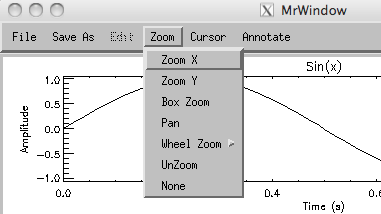
\includegraphics[width=0.75 \textwidth]{./figures/Zoom-Menu.png}
	\caption[Zoom Menu.]
	{Select an item in the zoom menu, then zoom.}
\end{figure}

%Add an image
\subsection{Add an Image to any Location}

\begin{lstlisting}
x = findgen(256)
y = findgen(256)
image = dist(256)
myWindow -> Image, image, x, y, LOCATION=[2,1], CTINDEX=17, /SCALE, /IMAXES, $
                                    TITLE='Dist(256)', XTITLE='X Title', YTITLE='Y Title'
\end{lstlisting}

\begin{figure}[h!]
	\centering
	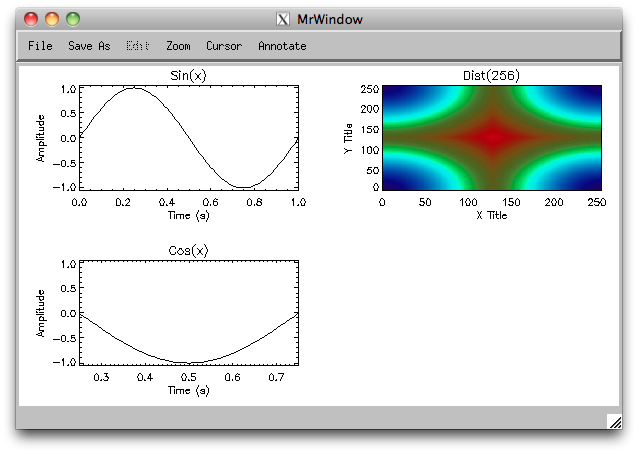
\includegraphics[width=0.5 \textwidth]{./figures/Add-Image.png}
	\caption[Add and Image.]
	{An image has been added to column 1 and row 2.}
\end{figure}

%Adjust Layout
\subsection{Alter Layout}

\begin{lstlisting}
myWindow -> SetProperty, XMARGIN=[10,15], XGAP=8, YGAP=6, /DRAW
\end{lstlisting}

\begin{figure}[h!]
	\centering
	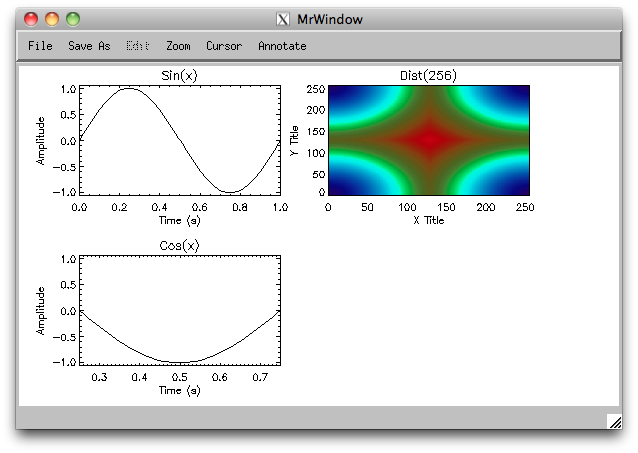
\includegraphics[width=0.5 \textwidth]{./figures/Adjust-Layout.png}
	\caption[Adjust the Plot Layout.]
	{The margins and gaps between plots have been changed.}
\end{figure}

\subsection{Add Colorbar}

\begin{lstlisting}
myWindow -> Colorbar, [2,1], CTINDEX=17, RANGE=[min(image), max(image)], /RIGHT, /DRAW
\end{lstlisting}

\begin{figure}[h!]
	\centering
	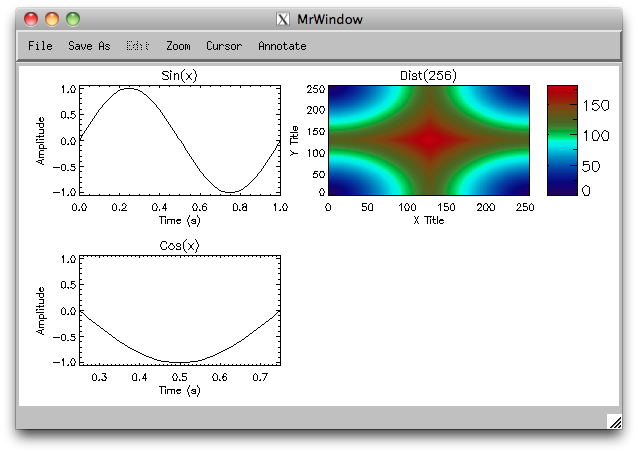
\includegraphics[width=0.5 \textwidth]{./figures/Add-Colorbar.png}
	\caption[Add a Colorbar.]
	{A colorbar has been added to the right of the image.}
\end{figure}

\subsection{Color Zoom}

\begin{lstlisting}
;Figure out the indices at which the objects are located
myWindow -> whichObjects
\end{lstlisting}
    
Get their object references and bind them

\begin{lstlisting}
myWindow -> GetProperty, 0, /IMAGE, OREF=oImage
myWindow -> GetProperty, 0, /COLORBAR, OREF=oCB
myWindow -> Bind, oImage, oCB, /CAXIS
\end{lstlisting}
    
    ;Turn on "Focus" from the "Cursor" menu
    ;Turn on "Wheel Zoom: Color" from the "Zoom | Wheel Zoom" menu
    ;Click on the image
    ;Make a scroll event with the mouse wheel
    
\subsection{Add \emph{Any} Plottable Object}

\begin{lstlisting}
x = findgen(101)/100
y = x^2
myPlot = obj_new('MrPlotObject', x, y, TITLE='y = x^2', XTITLE=x, YTITLE='y')
myWindow -> addPlots, myPlot, /DRAW
\end{lstlisting}
 










\end{document}